\documentclass[12pt,a4paper,oneside,titlepage]{report}
\usepackage[utf8]{inputenc}
\usepackage[spanish]{babel}
\usepackage{tex/mi_estilo}
%\usepackage[version=4]{mhchem}

\usepackage{hyperref}
\hypersetup{
    colorlinks=true, %set true if you want colored links
    linktoc=all,     %set to all if you want both sections and subsections linked
    linkcolor=blue,  %choose some color if you want links to stand out
    linktocpage
}

\author{Carlos Molina Ordóñez}
\date{20 de Marzo de 2017}
\title{Layout de un canal de lectura multi-paralelizado para un sensor de imagen CMOS}

\begin{document}
\maketitle
\tableofcontents
\listoffigures

\chapter{Introdución}\label{cap:intro}

\paragraph{}
En este trabajo se va a estudiar el proceso de diseño de un bloque fundamental
en cualquier sensor de imagen CMOS, el canal de lectura, que es el encargado
de convertir la información física recibida, que en esencia es el número de fotones
captados cada pixel, a una señal electrónica analógica que posteriormente será digitalizada,
procesada y, eventualmente, almacenada.

\paragraph{}
El estudio se va a centrar principalmente en el layout de este canal de
lectura y en todos los aspectos a tener en cuenta a la hora de abordar esta tarea.
El layout de un sistema microelectrónico consiste en su implementación física
sobre una oblea de algún material semiconductor, típicamente silicio cristalino. El
diseño de layout está sujeto a una serie de normas y problemas que iremos tratando
con mayor detenimiento a lo largo de la exposición.

\paragraph{}
Para introducir al lector en la materia será necesario describir, aunque sea
brevemente, conceptos sobre sensores de imágen, tecnología CMOS y explicar de manera
sencilla la arquitectura de un canal de lectura habitual.

\paragraph{}
Posteriormente se pasará a analizar en detalle los problemas y cuestiones que se
plantean a la hora de diseñar el layout de bloques analógicos en general,
centrándonos en última instancia en los que afectan directamente a un canal de lectura.

\section{Sensores de imagen}\label{cap:image_sensors}

\paragraph{}
Un sensor de imagen o cámara fotográfica es, en esencia, un sistema que capta
una imagen instantánea de una escena mediante la luz que emiten los objetos que
se encuentran en su campo de visión y que llegan a una pantalla donde se almacena
la información que proyecta ese rayo de luz, ya sea por un proceso químico
o electrónico, que es el caso que se va a tratar aquí.

\paragraph{}
En cuanto a los sensores de imágenes electrónicos se pueden distinguir dos tipos
principalmente, los CCD (\textit{Charge-Coupled Device}) y los CMOS
(\textit{Complementary Metal-Oxide-Semiconductor}). Las diferencias entre ellos
se basan en la tecnología empleada y en la forma de leer el array de pixeles.

\paragraph{Sensores de imágen CCD}
El concepto fundamental de un sensor de imagen CCD se basa en el almacenamiento
y propagación de los electrones fotogenerados en cada pixel. Mediante el efecto
fotoeléctrico, un fotón que impacte en la zona de silicio fotosensible, si tiene
la energía adecuada, arrancará un electrón desde la banda de valencia hasta la
banda de conducción, y podrá moverse libremente o arrastrado por campos eléctricos.

\paragraph{}
La carga almacenada en cada pixel será función lineal de la intensidad lumínica
captada por cada pixel. Tras la exposición, las cargas almacenadas en cada pixel
se irán transmitiendo al pixel inferior, y, de la misma forma que ocurre en un
registro de desplazamiento, la información de todos los pixeles se va transmitiendo
de unos a otros, hasta que al final todo el array es leído.\cite{Nakamura2005}

\paragraph{Sensores de imágen CMOS}
La diferencia fundamental de éstos con los sensores CCD es que los CMOS usan un
amplificador integrado en el píxel, a lo que nos referimos como APS (\textit{Active Pixel Sensor})
\cite{Fossum1993}. Ésto les da algunas ventajas
frente a los CCD, por ejemplo, sufren de menor efecto de ``blooming'', que podría
traducirse como deslumbramiento o destello, es decir, manchas blancas que pueden
producir los puntos muy brillantes a su alrededor por un desbordamiento de los
electrones fotogenerados en una zona. Podemos ver un ejemplo en la
imágen \ref{fig:blooming}\cite{Commons:Kriplozoik}.

\begin{figure}[h]
	\centering
	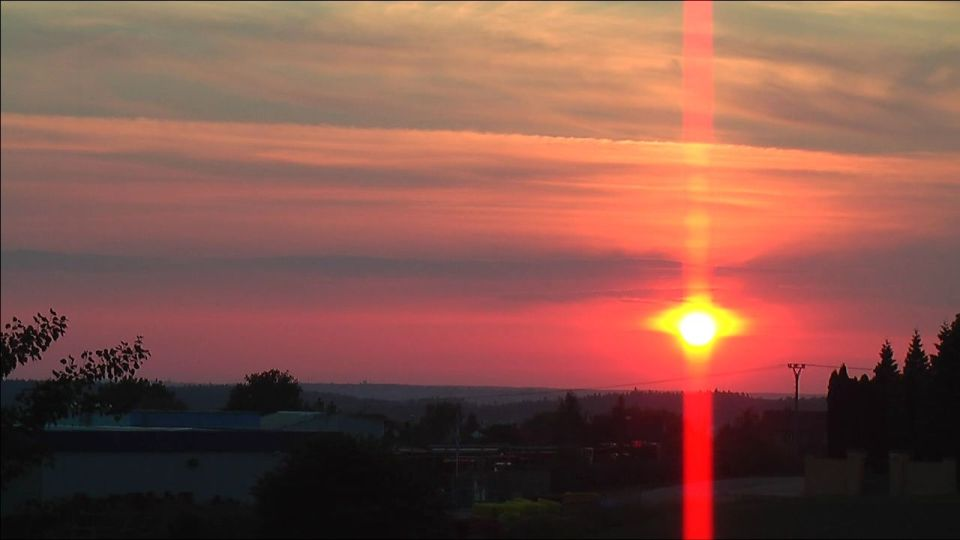
\includegraphics[width=0.4\textwidth]{img/blooming.jpg}
	\caption{Ejemplo de imágen con efecto de blooming en los píxeles brillantes}
	\label{fig:blooming}
\end{figure}

Otra ventaja es que pueden llegar a ser más rápidos y más baratos, ambos debidos
a la tecnología CMOS. Gracias a esto, hoy en día cada vez son más comunes que los
CCD.

\section{Arquitectura de sensores de imagen CMOS}

\subsection{Array de píxeles}\label{cap:pxa_array}

\paragraph{}
El dispositivo principal en un sensor de imagen es el píxel, que es el elemento
receptor de la luz y el encargado de hacer la primera conversión de fotones a
electrones. Estos fotones se traducen en electrones por medio del efecto fotoeléctrico
descrito por Albert Einstein: Cada fotón que incida en la superficie del silicio
es capáz de dar la energía suficiente a un electrón de la banda de valencia para que
pase a la banda de conducción y se pueda mover libremente por la red cristalina.
Si ahora aplicamos un campo eléctrico podemos guiar a todos los electrones
fotogenerados hacia un pozo de potencial donde almacenarlos temporalmente. Este
es el llamado proceso de exposición, que tiene una duración definida. En función
del tiempo de exposición y de la intensidad lumínica recibida por el pixel, este
se cargará con mayor o menor número de electrones.

\paragraph{}
El array de píxeles es la matriz compuesta de todos los píxeles organizados en filas
y columnas dónde la imagen formada por el sistema de lentes focalizará la imagen.
Habitualmente, los píxeles son cuadrados con un lado de unas 5 a 10 $\mum$, y el
array puede tener resoluciones de miles de píxeles en ambas dimensiones, lo que
significa que el array puede unos ocupar pocos centímetros, lo que lo convierte
habitualmente en el bloque más grande de todo el diseño.

\paragraph{}
En éste estudio vamos a trabajar con un array QSXGA de 2560 columnas por 2048 filas,
que tiene una relación de aspecto 5:4. Además de los píxeles activos, en un sensor
de imagen, habitualmente se incluyen algunos píxeles dummy, esto es, que no van
a ser incluidos en la imagen leída. Su función es la de evitar que los píxeles
en el borde tengan un entorno diferente al resto de píxeles del interior, lo que
puede alterar sus características.

\paragraph{}
Además de los píxeles dummy, habitualmente se incluyen algunos de los llamados
píxeles oscuros, píxeles iguales a los activos salvo porque no van a recibir luz
por construcción. Ésto se hace tapando el fotodiodo con los metales superiores,
sin modificar el resto de estructuras y transistores. El objetivo de estos píxeles
oscuros es ayudar en la calibración de los sensores una vez fabricados. Si
leemos píxeles que están tapados obtenemos el verdadero valor de negro y podemos
cuantificar el ruido debido al píxel y al canal, mejorando el ruido
que pudiéramos medir tomando una imágen en una habitación oscura, por ejemplo.

\paragraph{}
El sensor que estamos estudiando tiene $2560\times2048$ píxeles activos, 64 columnas
oscuras, con 4 píxeles dummy a cada lado de los píxeles activos y oscuros.
En cuanto a las filas, tendremos 8 filas oscuras en la parte inferior del array,
flanqueadas por 4 filas dummy arriba y abajo, al igual que alrededor de las filas
activas. Además se incluye una fila de test que servirá para la calibración simulando
que la fila en cuestión ha recibido una señal concreta. En la figura
\ref{fig:pxa_array}\footnote{Imágen obtenida del artículo de la bibliografía \cite{Jimenez-Garrido2012}},
se esquematiza todo lo dicho.

\begin{figure}
	\centering
	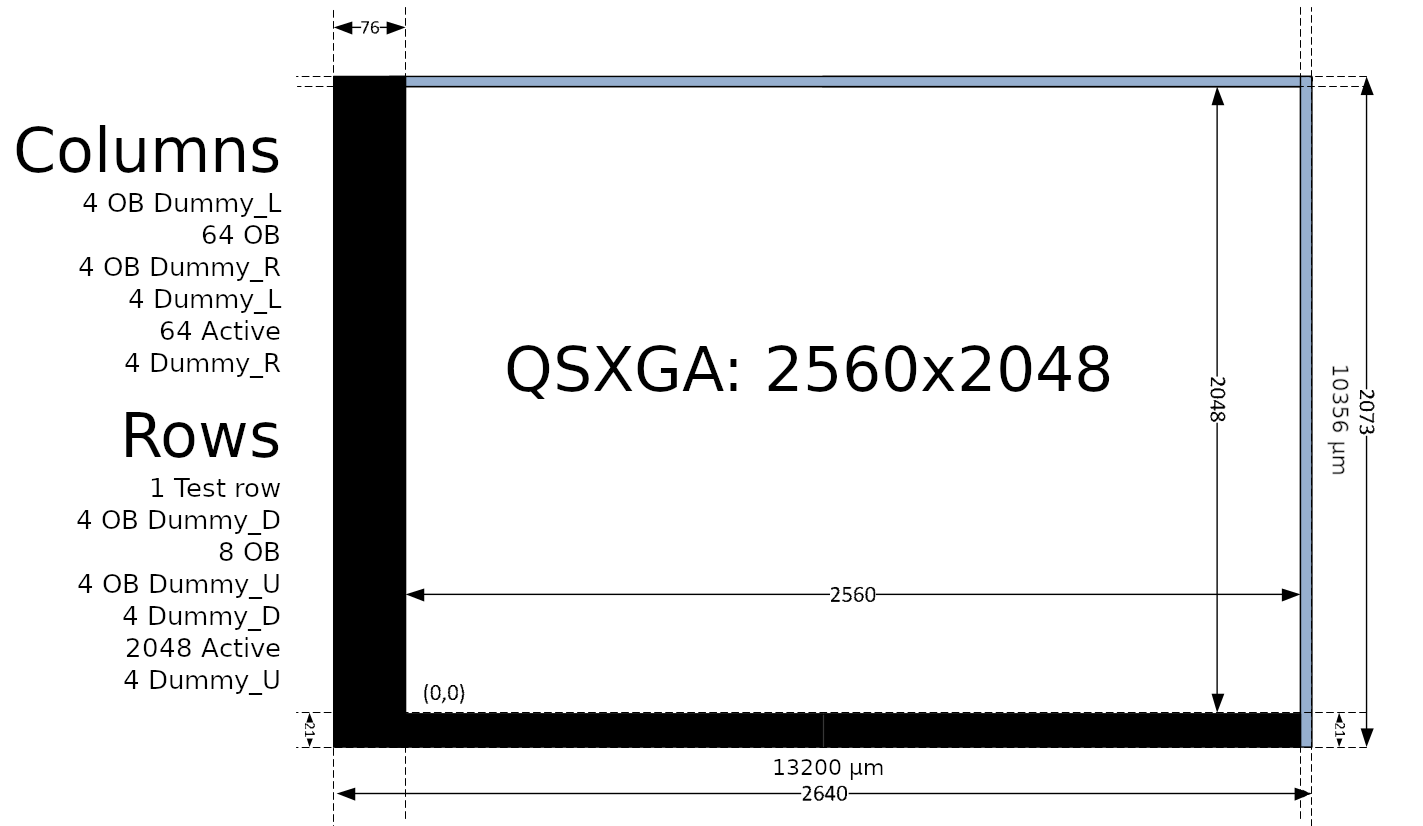
\includegraphics[width=0.9\textwidth]{img/pixel_array.png}
	\caption{Estructura del array de píxeles}
	\label{fig:pxa_array}
\end{figure}

\subsection{Canal de lectura}

\paragraph{}
El canal de lectura de un sensor CMOS, referido habitualmente por sus
siglas en inglés \textbf{RO} (\textit{Read-Out Channel}), es el bloque que se
encarga de traducir el voltaje almacenado en cada pixel durante el proceso
de exposición, en un número digital. Esta descripción concuerda con el concepto
ampliamente utilizado en electrónica de ADC, siglas en inglés de \textit{Analog-to-Digital
Converter}, (Convertidor Analógico-Digital), que, en general toma una señal
analógica y la expresa en valores discretizados.

\subsection{Otros bloques}

\paragraph{Ana ctrl row}. Este bloque se encarga del control analógico de las
señales que excitan en array por filas. Se sitúa a la izquierda y/o derecha del
array.

\paragraph{Pixel supply}. Es el bloque anaólgico que se sitúa en la parte superior
del array de píxeles y que provee la alimentación del array
y en ocasiones también provee señales que se distribuyan de forma vertical.

\paragraph{Referencias}. Es un bloque que se encarga de generar tensiones y corrientes
de polarización para el resto de bloque de forma que sean independientes de la
temperatura, fuente de alimentación y otros ruidos.

\paragraph{Serializador}. En el bloque digital que se encarga de ordenar y serializar
los datos de salida del canal de lectura para que puedan ser enviados al exterior del
chip por los puertos de salida serie.

\paragraph{Control Main}. Es el bloque digital encargado del control de todas las
señales y procedimientos que el sensor debe realizar para tomar una imágen, digitalizarla,
y enviarla al exterior.

\chapter{Tecnología CMOS}\label{cap:tecnologia_cmos}

\section{Introducción}\label{cap:intro_cmos}

\paragraph{}
La tecnología CMOS, que es ampliamente utilizada en el diseño de circuitos integrados
en la actualidad, se basa en la posibilidad de integrar en un mismo substrato
semiconductores con ambos dopados (\textit{n} y \textit{p}). Con ello podemos implementar transistores
MOSFET tanto PMOS como NMOS en un mismo diseño.

\paragraph{}
Es una tecnología que cumple ya los
50 años, debido a que empezó a ponerse en práctica a mediados de los años 1960.
Inicialmente se usó principalmente en circuitos digitales, debido a que los
transistores CMOS solo consumen potencia cuando conmutan, a diferencia de los
transistores de unión bipolar. Por otra parte, es más sencillo disminuir su tamaño
y tienen un menor coste de fabricación.

\paragraph{}
Poco a poco se fue introduciendo la tecnología CMOS en el diseño de circuitos
analógicos. Los bajos costes y la posibilidad de crear circuitos digitales y
analógicos en el mismo chip hacían esta opción muy interesante. Pero aún así, los
transistores bipolares eran mucho menos ruidosos y más rápidos que los MOSFET, por
lo que la trancisión fue lenta. Con el desarrollo de la tecnología CMOS, la velocidad
y el ruido de éstos, se ha visto muy mejorada, y actualmente domina el mercado,
aunque en muchos casos se sigue usando tecnología bipolar.
%WARNING
% Mirar un poco más esto (Historia y actual uso de las tecnologías del silicio)


\section{Proceso de fabricación}\label{cap:fabricacion}

\paragraph{}
La gran mayoría de los circuitos integrados CMOS están construidos sobre silicio.
El silicio (Si), elemento de número atómico 14, es muy abundante en la Tierra, aunque
no se encuentra de forma pura, sino como óxidos de silicio o silicatos. Entre los
óxidos de silicio, basados fundamentalmente en la sílice o dióxido de silicio
(SiO\textsubscript{2}), se encuentran el cuarzo y el sílex, ambos ampliamente extendidos
en la corteza terrestre. Los silicatos son sales basadas en el ión silicato (SiO\textsubscript{4}),
y forman parte de minerales como los feldespatos, micas, berilio.

%WARNING
%Leer algo en el libro de minerales y rocas en casa

\paragraph{}
A pesar de estar en tan alta abundancia en la Tierra, como se dijo antes, el silicio
puro no se dá naturalmente, debe ser refinado y cristalizado. El proceso consiste,
tratado de manera sencilla, en extraer el óxigeno de los compuestos mencionados arriba
a base de añadir carbono y fundir la mezcla en un horno. Tras éste y otros procesos
obtendríamos silicio relativamente puro, pero en forma policristalina (habitualmente
nos referiremos a éste como polisilicio o \textit{poly} por su abreviatura inglesa).
Esta forma contiene silicio puro, pero
cristalizado en pequeños cristales independientes con diferentes planos cristalinos
creando efectos de borde en el interior del conglomerado, que anulan las cualidades
semiconductoras del silicio.

\paragraph{}
Para construir un único monocristal de silicio se suele usar el llamado proceso
de Czochralski, en el cual, una varilla de silicio usada como semilla se va
rotando en un baño de silicio puro fundido a unos 1400\centigrade C de manera que va creciendo
en diámetro a medida que los átomos se silicio se van depositando en la capa externa.
Esta técnica fue introducida por Jan Czochralski en 1915
%WARNING
%Decir algo mas

\paragraph{}
Lo que queda es un lingote de aproximadamente un metro de largo y pocas decenas
de centímetro de diámetro de silicio monocristalino siguiendo la estructura cristalina del
diamante.

\paragraph{}
Para ser usado en la industria de semiconductores, estos lingotes se deben laminar
en obleas de pocos milímetros de espesor sobre las que se implementarán los
circuitos integrados, que se suelen distribuir en una matriz ocupando toda la
superficie de la oblea que luego será cortada para separar cada "dado".

\paragraph{}
Con estos procesos tendríamos tan solo el substrato de silicio sobre el que
se debe construir el circuito, los transistores y otros dispositivos que se
necesiten. Esto se hace mediante fotolitografía, una técnica que permite
construir cada capa mediante la projección de luz ultravioleta a través de
unas máscaras que permiten o no pasar la luz según el layout diseñado.

\paragraph{}
Para empezar se recubre toda la oblea con un material fotosensible a la luz UV,
que dependiendo de si recibe luz o no, cambia sus propiedades haciendo que donde
ha recibido luz pueda ser eliminado posteriormente y quedar sólo donde no se recibió
luz, o viceversa. De esta forma obtenemos un recubrimiento selectivo con este
material, haciendo que, en un paso posterior podamos hacer crecer, sobre las zonas
sin recubrimiento, una capa de óxido de silicio si queremos un aislante, o de polisilicio,
cuyos usos se tratarán más adelante, o de metal como conductor, habitualmente
aluminio o cobre, o algún tipo de dopado para crear las difusiones por ejemplo.

\paragraph{}
Tras las creación de cada capa, en la mayoría de los casos se realiza un pulido
fino de la superficie para que la siguiente capa asiente correctamente sobre una
superficie plana.

\paragraph{}
Todo el proceso de fabricación se puede consultar con más detalle en la bibliografía,
en el libro de Hastings \cite{Hastings2001:fabrication}.

\section{Transistores CMOS}\label{cap:transistor_cmos}
\paragraph{}
El dispositivo fundamental que usa en cualquier circuito integrado CMOS es el
transistor CMOS, ya que es la base de funcionamiento de circuitos tanto digitales
(puertas lógicas, inversores, flip-flops, buffers), como de circuitos analógicos
(amplificadores operacionales y de transconductancia, convertidores analógico-digital,
referencias de tensión, bandgap).

\paragraph{}
El transistor CMOS es un dispositivo electrónico de 3 terminales que se basa
en una estructura MOS (Metal-Óxido-Semiconductor). En esta estructura, sobre un
substrato semiconductor se asienta una capa de \textit{óxido} aislante y sobre ella un
material metálico, que en las tecnologías actuales suele tratarse del polisilicio
que se mencionó anteriormente. La capa de óxido fino, tiene un espesor muy pequeño,
y debe controlarse mucho en la fabricación, ya que variaciones en su grosor, daría
lugar a modificaciones de la capacidad de puerta.

\paragraph{}
Usando la estructura vertical \textbf{M}etal-\textbf{Ó}xido-\textbf{S}emiconductor,
se puede construir un transistor creando a ambos lados de ella, zonas de silicio
altamente dopado donde contactaremos dos terminales, que llamaremos \textit{fuente} o \textbf{S}
(\textit{source}), y \textit{drenador} o \textbf{D} (\textit{drain}). En la capa superior
del polisilicio colocaremos el terminal llamado \textit{puerta} o \textbf{G} (\textit{gate}).
En la figura \ref{fig:nmos} podemos ver la estructura física de este dispositivo.

\paragraph{}
Cuando se aplica un voltage en puerta, el óxido fino crea un
condensador entre el polisilicio y el substrato semiconductor. De esta forma,
electrones presentes en substrato son atraídos hacia la superficie del substrato,
lo que facilita la creación de un canal, que permitirá la circulación de una
corriente entre las dos difusiones fuente y drenador. Cuando la tensión en la puerta
es menor que cierto valor, la creación del canal no se dá, y los terminales D y S
quedan eléctricamente aislados.

\paragraph{}
La dimensión de la puerta en la dirección que une drenador y fuente se llama
''longitud'', notada como \textbf{L}. La otra dimensión de la puerta, perpendicular a ésta
se llama ''anchura'', abreviada como \textbf{W}

\paragraph{}
Como mencionamos al principio, también podemos crear transistores PMOS en estas
tecnologías. Se hace fabricándolos dentro de un pozo N, esto es, una zona
donde el substrato tipo-p original, se ha dopado de forma que se consigue un substrato
tipo-n. El transistor embebido en este pozo tiene, entonces, la misma estructura,
salvo que las difusiones para drenador y fuente son con dopado positivo \textbf{P+}.
Una representación de este tipo de transistor puede verse en la figura \ref{fig:pmos}.

\begin{figure}
	\centering
	\begin{subfigure}[b]{0.45\textwidth}
		\includesvg[width=\textwidth]{svg/nmos.svg}
		\caption{NMOS}
		\label{fig:nmos}
	\end{subfigure}
	~ %add desired spacing between images, e. g. ~, \quad, \qquad, \hfill etc.
	%(or a blank line to force the subfigure onto a new line)
	\begin{subfigure}[b]{0.45\textwidth}
		\includesvg[width=\textwidth]{svg/pmos.svg}
		\caption{PMOS}
		\label{fig:pmos}
	\end{subfigure}
	\caption{Representación física de transistores MOS en tecnología CMOS}
	\label{fig:cmos_transistors}
\end{figure}

\section{Otros dispositivos en tecnología CMOS}\label{cap:otros_dispositivos}

\paragraph{}
Usando la misma tecnología es posible disponer en el mismo diseño otros dispositivos
además de los mencionados transistores.

\subsection{Resistencias}
\paragraph{}
En todo diseño microelectrónico resulta prácticamente indispensable en algún
momento el uso de algún elemento resistor pasivo. Estos dispositivos podemos
crearlos usando la resistividad que ofrecen algunos de los materiales que se emplean
en el diseño. En ocasiones puede usarse el sustrato de silicio, o un pozo NWELL, pero
una de las técnicas más habituales es usar el silicio policristalino o \textbf{polisilicio}.

\begin{figure}[h]
	\centering
	\includesvg[width=0.6\textwidth]{svg/poly_res.svg}
	\caption{Estructura física de una resistencia de polisilicio}
	\label{fig:poly_res}
\end{figure}

\paragraph{}
Para construir una resistencia de polisilicio (\ref{fig:poly_res}) se crea una tira de polisilicio
que se deposita sobre una capa de oxido de campo, conectando sus dos extremos con
un contacto a la primera capa de metal. Cómo vemos, esto se parece a la capa de
polisilicio que se usa para construir un transistor CMOS. Pero existe una diferencia
fundamental. El óxido sobre el que se deposita el poly, en este caso, es \textit{oxido de
campo}, más grueso y menos preciso que el \textit{óxido fino} de los transistores.

\subsection{Condensadores}\label{cap:condensadores}
\paragraph{}
Los condensadores son otro elemento fundamental en muchos diseños analógicos. Un
condensador, como sabemos, consiste en dos placas conductoras separadas por una pequeña
distancia, que almacena carga eléctrica en cada terminal.

\paragraph{}
En el contexto que nos ocupa, tenemos varias opciones para fabricar un condensador:

\paragraph{poly}
Llamaremos así al condensador que creamos con una lámina de polisilicio sobre una
capa de óxido fino, que en función de la tecnología, puede tener varios espesores
definidos por el fabricante. Un terminal sería el poly, y el otro el substrato.

\paragraph{metal-metal}
Entre las diferentes capas de metal tenemos varias posibilidades de crear un condensador
también. Normalmente los fabricantes definen unos cuantos tipos. Pueden tratarse de
dos láminas rectangulares a diferentes alturas, o, por ejemplo, dos peines que
entrelacen sus dedos de forma alternativa.

\paragraph{mos}
Por último, podemos usar la capacidad de puerta que siempre tiene un transistor MOS
para crear un condensador. Un terminal sería la puerta, y el otro sería el cortocircuito
de drenador, fuente y sustrato. La principal ventaja de éstos es que su capacidad por
unidad de área suele ser elevada debido al pequeño espesor del óxido de puerta. Por contra,
tienen la desventaja de presentar un comportamiento no lineal, ya la que la capacidad
depende del punto de operación del transistor.

%WARNING
%Algo más? (gráfico capacidad-Vg?)

\subsection{Diodos}\label{cap:diodos}
\paragraph{}
Una forma de crear diodos en esta tecnología es crear una zona de dopado N (difusión N+)
junto a una zona con dopado P (difusión P+). Es habitual dibujar uno de los dos terminales
			en forma de anillo rodeando al otro terminal. Fig \ref{fig:diodo}:

\begin{figure}[h]
	\centering
	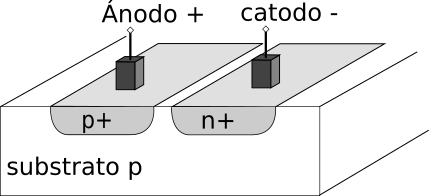
\includegraphics[width=0.4\textwidth]{img/diodo.png}
	\caption{Estructura física de un diodo de unión PN}
	\label{fig:diodo}
\end{figure}

\subsection{Transistores bipolares}\label{cap:bipolares}
\paragraph{}
También se pueden crear transistores de unión bipolar a partir de la creación
de dos uniones PN enfrentadas. En el caso de tener substrato P podemos conseguir
de forma sencilla un transistor tipo \textbf{PNP}, creando un contacto al substrato
P para el Colector (C), un pozo N dónde se crea un contacto a N+ para la base (B), y
una difusión positiva P+ dentro del pozo N, que funcionará como emisor (E).
Véase la figura \ref{fig:pnp}:

\begin{figure}[h]
	\centering
	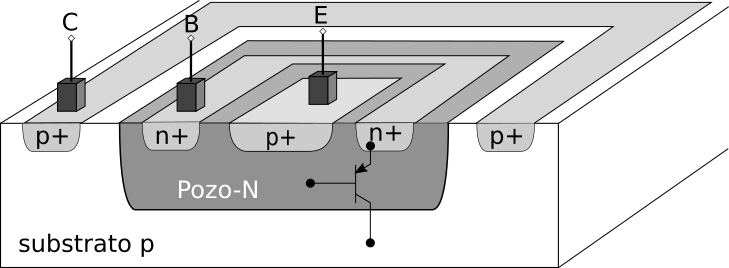
\includegraphics[width=0.7\textwidth]{img/pnp.png}
	\caption{Estructura física de un transistor de unión bipolar PNP}
	\label{fig:pnp}
\end{figure}

\paragraph{}
Crear un transistor NPN en una tecnología de substrato P es algo más complicado,
pero afortunadamente, existe la posibilidad de crear una estructura especial, que
va a ser muy usada en algunos casos con diferentes finalidades. Se trata del
llamado \textit{pozo N profundo} (\textit{Deep-N-Well} en inglés), que no
es más que un pozo N enterrado baja una capa de substrato P, que queda aislada del
substrato P del resto del chip si las uniones PN que forma con ambos substratos P,
están polarizadas inversamente.

\paragraph{}
De ésta forma podemos crear un transistor NPN entre el substrato profundo N,
colector (C), el substrato P encerrado por el anterior, base (B), y una difusión
N+ en el centro de este substrato P, que funcionará como emisor (E). Véase la
figura \ref{fig:npn}:

\begin{figure}[h]
	\centering
	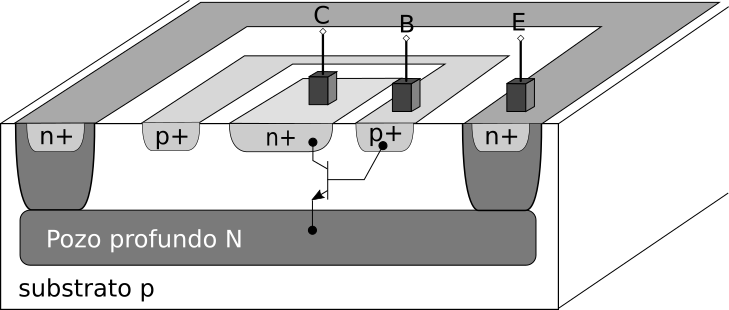
\includegraphics[width=0.7\textwidth]{img/npn.png}
	\caption{Estructura física de un transistor de unión bipolar NPN}
	\label{fig:npn}
\end{figure}

%WARNING
%Aniadir si es posible algun otro dispositivo en tecnologia CMOS

\section{Diseño de layout}\label{cap:layout}

\paragraph{}
El término \textit{layout} hace referencia a la implementación física del circuito
electrónico que se quiere fabricar. El layout consiste en un dibujo con toda
la información que necesita la empresa fabricante para implementar el circuito
sobre la oblea de silicio. Dicha información se representa por medio de "capas"
que se distribuyen en un espacio bidimensional. Cada capa tiene un significado y
unas normas que cumplir. El trabajo del diseñador de layout es definir, dibujar y
verificar el layout de los diferentes bloques que componen el chip siguiendo
las normas dadas por el fabricante, y procurando el mejor funcionamiento posible
del circuito en el menor area que le sea posible.

Como veremos más adelante, el diseño del layout de un circuito afecta o puede afectar
mucho al funcionamiento final del mismo.

\subsection{Capas de layout}\label{cap:capas_layout}

\paragraph{}
Todo diseño de layout está compuesto de una cierta cantidad de capas, de las cuales
algunas tienen significado físico directo y otras son capas que usa el software de
diseño para verificaciones o para cambiar propiedades de otras capas.

\paragraph{}
Naturalmente, los nombres de estas capas están asignados por cada fabricante en
concreto, pero los nombres que presento aquí para describirlas son los que usaré
para identificarlas durante el resto del documento.

\paragraph{NWELL}
Esta capa define el pozo N en una tecnología de substrato P. En ella se deben
situar los transistores PMOS y normalmente se polariza mediante difusiones \textbf{P+}
a la tensión más alta del circuito (VDD o similar).

\paragraph{WB}
Esta capa define el pozo enterrado (del inglés \textit{Well Buried}), o también
llamado pozo profundo (\textit{Deep-N-Well}), y como se introdujo en el capítulo
\ref{cap:bipolares}, donde se usaba para crear transistores bipolares. Esta
estructura también puede ser usada para crear zonas de substrato P aisladas del substrato
P del resto del chip. Dentro de esta zona se pueden disponer, por ejemplo, circuitos
CMOS digitales, con objeto de aislar el ruido que puedan generar a circuitos analógicos
cercanos.

\paragraph{XN}
Zona de difusión con dopado negativo N+, estará en las difusiones de drenador/fuente
de los transistores NMOS y en los contactos a substrato de los pozos N.

\paragraph{XP}
Zona de difusión con dopado positivo P+, de manera complementaria a la XN,
se usará para las difusiones de drenador/fuente
de los transistores PMOS y para los contactos al substrato P.

\paragraph{ACTIVE}
La capa activa indica al fabricante las zonas en las que se debe eliminar el óxido grueso (óxido
de campo). Ésto lo haremos siempre que haya que contactar una zona de difusión N o P,
o queramos crear la puerta de un transistor como se explica en el siguiente párrafo.

\paragraph{GC}
Zona donde se creará una capa de polisilicio o (\textit{poly}). Si coincide con capa activa,
se crearán puertas de transistores sobre una fina capa de óxido de silicio,
al cual llamaremos \textit{óxido de puerta}.
En los lugares donde no coincida con area activa se construirá sobre oxido grueso,
de espesor no tan controlado, y se usará para rutar líneas o para crear resistencias
de poly.

\paragraph{CS}
Contacto. Normalmente son cuadrados que definen contactos entre el Metal 1 y el
polisilicio (si están, respectivamente, sobre M1 ó GC), o al substrato, teniendo que
usar la capa ACTIVE para poder bajar al substrato.

\paragraph{M1}
Metal 1. Es el primero de los metales y se suele usar para contactar
transistores entre sí y con otros dispositivos, o para crear anillos de contactos
a substrato.

\paragraph{M2-M3-...-(M5)}
Otros metales. En función de la tecnología, pueden ser
más o menos capas de metal, por ejemplo 4 ó 6. La última capa de metal puede ser
diferente, ser más gruesa y menos resistiva, con objeto de usarse como caminos de
alimentación, que deben soportar corrientes mayores. Habitualmente, para seguir un órden
y ayudar al rutado del circuito, se suele definir un criterio de direcciones
en función de si la capa de metal es par o impar se dispondrán verticales u
horizontales. Mientras no se diga lo contrario, en el texto se usará el criterio
horizontal = impar, vertical = par.

\paragraph{V2-V3-...-(V5)}
Vías. Crean conexiones verticales entre un metal y el
inmediato superior. Se suelen usar varios para cada conexión por evitar una
posible rotura y para disminuir la resistencia total.

\paragraph{SA}
Del vocablo inglés \textbf{salicide}, que es una contracción de "\textbf{s}elf-\textbf{a}ligned si\textbf{licide}",
ésto es, siliciuro auto-alineado. Siliciuro es cualquier compuesto binario de
Silicio con otro elemento, generalmente metal; por ejemplo: CoSi\textsubscript{2}
ó TiSi\textsubscript{2}. Este siliciuro se dice auto-alineado porque el metal que
se deposita sobre el chip durante el proceso de fabricación se adhiere sólo sobre
dónde hay silicio (o poly), y no donde ya se ha hecho crecer la capa de óxido.
La reacción del silicio con el metal crea el siliciuro, lo que crea una capa más
conductiva que el silicio puro \cite{Maex:silicides}.

\paragraph{}
Por defecto todos el poly y las difusiones van silicidadas, pero usando la capa \textbf{SA},
podemos indicar que no se deposite siliciuro sobre algunas zonas, para, por ejemplo,
permitir que las resistencias de poly sean más resistivas.

\subsection{Herramientas de CAD}

\paragraph{}
Las herramientas de CAD (\textit{Computer Assisted Design}) se usan
en muchos campos de la ingeniería o la arquitectura, y actualmente, debido a la alta
complejidad de los diseños son de uso prácticamente obligado.

\paragraph{}
En el caso que nos ocupa, el diseño de circuitos microelectrónicos,
tiene gran importancia el buen uso y conocimiento de las herramientas por parte de
diseñadores. En nuestro caso, estas técnicas tienen dos finalidades fundamentales:
el diseño y simulación eléctrica y, por otro lado, la implementación física. Entre ellas
hay muchas diferencias, pero también existe una inevitable relación de dependencia.
La implementación física viene definida por el diseño eléctrico, pero a su vez, como
veremos en muchos casos, éste último condiciona el diseño eléctrico.

\paragraph{}
Por otra parte, en microelectrónica, debemos tener presente que
hay una división importante entre dos ámbitos que son bastante diferentes en cuanto
al flujo de diseño, simulación e implementación física, aunque ambos se basan sobre
la misma tecnología. Me refiero a la separación entre el ámbito \textbf{analógico}
y el \textbf{digital}. En éste trabajo nos centraremos en la parte analógica
puesto que el canal de lectura es un bloque fundamentalmente analógico.

\paragraph{}
Considerando únicamente el layout, estos dos ámbitos, analógico y
digital son también bastante diferentes. En el caso del layout digital, el flujo
de trabajo, debido a la gran cantidad de dispositivos que habitualmente son necesarios
para diseñar cualquier bloque digital, está altamente automatizado por algoritmos
de distribución y rutado automático (\textit{place and route}). Mediante estas
herramientas, el diseñador digital de back-end implementa el layout de un bloque
digital que el diseñador de front-end ha diseñado para que tenga un funcionamiento
definido.

\paragraph{}
Las herramientas de \textit{place and route} consisten en algorítmos
de posicionamiento de los sub-bloques digitales que conforman un macro-bloque:
inversores, buffers, puertas lógicas, flip-flops... La herramienta, considerando el
rutado entre cada bloque, los posiciona y los interconecta de forma que los tiempos
de propagación de las señales entre ellos estén dentro de unos márgenes aceptables.
En ocasiones, esta implementación física da problemas por cuestiones de congestión
de rutado, o por problemas de \textit{timing}, las señales no se propagan con la
suficiente velocidad y ésto genera fallos en el funcionamiento general de bloque.
Por todo esto, es muy importante la simulación post-layout de los bloques digitales.
Éstas tienen en cuenta los tiempos de respuesta de los sub-bloques digitales, los cuales
han sido obtenidos previamente mediante simulaciones analógicas, o vienen dados por
el fabricante de la tecnología en unos ficheros que incluyen tiempos y capacidades de
sus nodos. Posteriormente la herramienta considera las capacidades de las líneas de
rutado entre los sub-bloques, mediante un extraído de parásitos. Con todo ésto
se obtiene una simulación bastante cercana al comportamiento real del bloque una vez
fabricado, aunque nunca se puede asegurar al cien por cien el correcto funcionamiento
de todo el chip, lo que genera chips defectuosos en cada oblea fabricada.


\paragraph{}
Para el caso analógico, el editor de layout consiste en un software
de diseño gráfico en 2 dimensiones, dónde el diseñador de layout va dibujando los
dispositivos, y los va interconectando mediante líneas de rutado en los diferentes
metales que tiene a su disposición. El proceso es mucho más manual que en el caso
digital, dada la relativa simplicidad de los circuitos analógicos, frente a los
digitales. Un bloque analógico es abordable por una persona en unos pocos días o
semanas, ayudándose obviamente, de herramientas de replicación, jerarquizado, celdas
prediseñadas o parametrizadas. El caso analógico también se realiza de forma más
manual debido a la naturaleza de las señales analógicas, al ser éstas, en algunos casos,
más susceptibles a ruidos ,interferencias o acoplos con otras señales.

\paragraph{}
En los circuitos puramente digitales, las señales cambian de un
valor alto (1) a un valor bajo (0), siendo menos importante el valor exácto
mientras éste se encuentre dentro de los márgenes definidos. Por el contrario,
en un circuito analógico, hay que tomar cuidado en diseñar un layout que preserve
los valores de las señales anlógicas y tenga un impacto mínimo en los tiempos de
propagación o asegurar que dos dispositivos o bloques que deban comportarse idénticamente
así lo hagan.

\subsection{Problemas habituales en el diseño de layout}

\paragraph{}
A continuación se van a exponer y explicar algunos de los problemas habituales que
afectan a cualquier diseño de layout y que el diseñador debe hacer frente para
resolver o minimizar mediante su experiencia y la ayuda de las herramientas, de CAD,
la simulación post-layout y los consejos del diseñador analógico del bloque en cuestión.

\subsubsection{Area}

\paragraph{}
La superficie sobre la que se diseña un chip es limitada, y además es
un factor en contra del beneficio económico que tendrá la fabricación y venta del
chip. A menor sea el area usada por el chip, más chips caben en cada oblea, que tiene
un precio constante, definido por el fabricante en función de la tecnología y otros
parámetros. Por lo tanto, como punto de partida, podemos concluir que \textbf{el área
es siempre un parámetro a minimizar}, a cualquier nivel de jerarquía.

\paragraph{}
Si bien esto es la idea general, también es verdad que no siempre es
la prioridad, o bien el área no supone un problema porque, por ejemplo, debido a la
distribución de los bloques, un bloque resulte disponer de area más que suficiente.
Puede darse el caso incluso de que se prefiera distribuir un circuito de manera más
holgada pero más uniforme, antes que arrinconar todo el circuito en una zona y dejar
espacio libre en otras zonas. Ésto, por ejemplo, podría ayudar a mejorar la correlación
entre dispositivos, o \textit{matching}.

\subsubsection{Mismatch}

\paragraph{}
El mismatch es un problema generalizado en muchos campos de
la ingeniería donde se requiere la construcción de dispositivos que se comporten
igual, y por problemas de fabricación u otros agentes externos se comportan ligeramente
diferente.

\paragraph{}
En el caso del layout el mismatch puede deberse al proceso de fabricación,
que puede crear dispositivos de \textbf{dimensiones ligeramente mayores o menores},
o otorgar al silicio propiedades ligeramente diferentes, como la \textbf{concentración de
dopado}, lo que puede hacer que unas zonas sean mas o menos conductivas o que varíen
parmámetros como la tensión umbral.

\paragraph{}
Otra forma de que se creen diferencias entre unos dispositivos y otros
independientemente de la fabricación, es por ejemplo por la \textbf{distribución irregular
de la temperatura} cuando el chip esté funcionando. Debido a la ley de Joule, cualquier
corriente circulando por un material, lo calentará en función de la densidad de corriente
que lo atraviese. Si en una zona del chip tenemos un bus de alimentación, o un circuito
que consuma mucha corriente, calentará la zona cercana, creando gradientes de temperatura.
Si tenemos dos circuitos o dispositivos, uno de ellos cerca y otro lejos de esta zona,
posiblemente no se comporten igual.

\paragraph{}
Para minimizar los efectos de los gradientes, se suelen usar estructuras
de centroide común, que en teoría, para gradientes lineales, logran el emparejamiento
perfecto. Por ejemplo, si tenemos un array lineal de dos tipos de dispositivos diferentes,
cada uno con una multiplicidad de 4, deberíamos usar una estructura ABBA$\vert $ABBA, en vez
de AAAA$\vert $BBBB, dónde A y B representan instancias del mismo dispositivo. En el primero
de los casos, si existe un gradiente lineal en la dirección del array, el efecto de éste
actuará en positivo en unos y en negativo en otros, de forma que el efecto en A se compensa
al efecto en B. En cambio en el segundo caso, como promedio, los A sufrirán el efecto
más o menos que los B.

\paragraph{}
Ésto se puede aplicar también para arrays bidimensionales de dispositivos,
de forma que se pueden usar estructuras como la que se muestra en la figura \ref{fig:centroide_comun}:

\begin{figure}[h]
	\centering
	\includesvg[width=0.7\textwidth]{svg/common_centroid.svg}
	\caption{Estructura de centroide común}
	\label{fig:centroide_comun}
\end{figure}

\paragraph{}
Algunas de las reglas que se recomienda seguir para un buen matching entre transistores
serían \cite{Hastings2001:mos_matching}:

\begin{enumerate}
	\item Usar dimensiones idénticas para los \textit{fingers} del transistor,
	esto es, cada uno de los transistores unitarios dispuestos en paralelo,
	que forman uno mayor.
	\item Maximizar el área ($L \times W$) de los transistores, ya que las
	variaciones relativas en tamaños son menores.
	\item Orientar los transistores en la misma dirección, ya que el silicio
	puede presentar alguna anisotropía inherente a la fabricación.
	\item Situar los transistores lo más cerca posible entre ellos. A mayores
	distancias, mayores pueden ser las diferencias de temperatura, dopado, ruido...
	\item Uso de estructuras de centroide común.
	\item A ser posible, uso \textit{dummies} en los contornos del
	array de transistores. Un transistor, o en general, dispositivo \textit{dummy},
	es idéntico a uno activo en cuanto a construcción física, pero conectado de
	forma que no actúa eléctricamente, por ejemplo, un transistor CMOS podría
	conectarse a tierra todos sus terminales.
	Con esto evitamos los posibles efectos de borde que afectan un dispositivo
	que no tiene menos vecinos que los del interior del array.
	\item Colocar los dispositivos lejos de dispositivos de potencia o lineas
	de alimentación que pueden generar fuertes gradientes de temperatura.
	\item Intentar no rutar metal sobre la zona activa de los transistores,
	aunque esto es en muchos casos inviable. En caso de tener que hacerlo, tratar
	distribuir el metal de la forma más simétrica posible, afectando a todos
	los dispositivos por igual.
\end{enumerate}

%WARNING
%Detallar estas buenas prácticas

\chapter{Diseño electrónico de un canal de lectura}\label{cap:ro_sch}

El canal de lectura es el circuito que lee la información almacenada en los píxeles
tras el tiempo de exposición.
En la arquitectura más habitual, y la que vamos a tratar en este estudio, los
píxeles se leen por columnas, entendiéndose que el chip tiene una dirección
\textit{vertical} y otra \textit{horizontal}. Siguiendo ese criterio, el canal de lectura se
sitúa debajo del array de píxeles de forma que cada columna del canal quede alineada
con cada columna del canal.\\

Idealmente podríamos usar un canal por columna, y meter en ese espacio todo el circuito
para la columna. Pero, en algunos casos, debido al pequeño tamaño de los píxeles
--- suelen tener unos 5, 8, 10$\mum$... --- resulta complicado o incluso imposible diseñar el
layout de dicha circuitería en ese reducido espacio horizontal.
Por esta razón, es una práctica común usar el \textit{pitch}\footnote{De ahora en adelante
usaremos la palabra inglesa \textit{``pitch''} para referirnos al espaciado con el
que se repite una estructura periódica como el canal de lectura o el array}
de varios píxeles, por
ejemplo 2 ó 4, y así tener más espacio para diseñar el layout del circuito. Por contra,
debemos apilar estos 2 ó 4 canales en filas, lo que veremos que nos trae algunos
problemas a la hora de diseñar el layout.\\

De ahora en adelante nos centraremos en el caso de un sensor cuyos píxeles tengan
un área de $5\mum \times 5\mum$, y en el que se apilan 2 canales para leer 2
columnas de píxeles. Por tanto, el ancho de un canal será de $10\mum$, encajando
exáctamente en la anchura de 2 columnas de píxeles.\\

\section{Estructura general}\label{cap:ro_sch_estructura}

El canal de lectura es un circuito analógico que va a convertir el voltaje
dado por el píxel tras haber sido expuesto a la luz durante un tiempo y
convertirlo en un valor analógico bien definido entre unos límites que van a
significar \textit{blanco} y \textit{negro}, con una resolución definida.\\

Por tanto, el canal de lectura es principalmente un ADC (en inglés, \textbf{A}nalog
to \textbf{D}igital \textbf{C}onverter, o convertidor analógico-digital).
Una arquitectura usada habitualmente es el convertidor de rampa.
Éste, para la conversión usa un generador de una rampa de voltaje que se usa para
comparar contra el valor dado por el píxel. Cuando ambos valores coinciden,
la salida del comparador cambia de estado mediante un flanco de subida o bajada.
De esta forma la conversión de un valor de tensión se traduce en la detección temporal
de un flanco.\\

De manera simultánea a la rampa analógica se lanza una rampa digital que va contando
valores desde 0 hasta un número que viene determinado por la resolución, y que va a
evolucionar a la misma velocidad que la analógica. Posteriormente, un circuito digital
detectará el flanco y parará el reloj de la cuenta digital, obteniéndose de esta forma
un valor digital para el valor analógico leído.\\

Entre las ventajas de usar un convertidor de rampa frente a otras muchas posibilidades
que existen en la literatura para convertir valores analógicos a digitales, podemos
destacar las siguientes:\\

\begin{enumerate}
	\item Se trata de un circuito muy simple, que puede reducirse a un comparador
	creado con un OTA simple de 5 transistores, más un par de condensadores y
	algunas llaves. Cualquier otra arquitectura (convertidor SAR, sigma-delta...)
	implica muchos más transistores y posiblemente más consumo.
	\item Se puede obtener una buena linealidad si se diseña una buena rampa
	y se hace operar al comparador en un punto de operación similar en todos los casos,
	consiguiendo ecualizar los tiempos de transición del mismo.
	\item Es fácilmente repetible en todas las columnas, ya que podemos separar
	la generación de la rampa de los comparadores.
\end{enumerate}

\section{Operación de lectura}\label{cap:ro_sch_operacion}

Para abordar el diseño de un canal de lectura debemos entender como se realiza la
operación de lectura de los píxeles.
En la figura \ref{fig:pixel} podemos ver el esquemático del píxel 5T
que vamos a usar para este estudio. El fotodiodo (PD), es el elemento que más
área ocupa del píxel, ya que es el area que recibe los fotones.

\begin{figure}[h]
	\centering
	\begin{subfigure}{0.6\textwidth}
		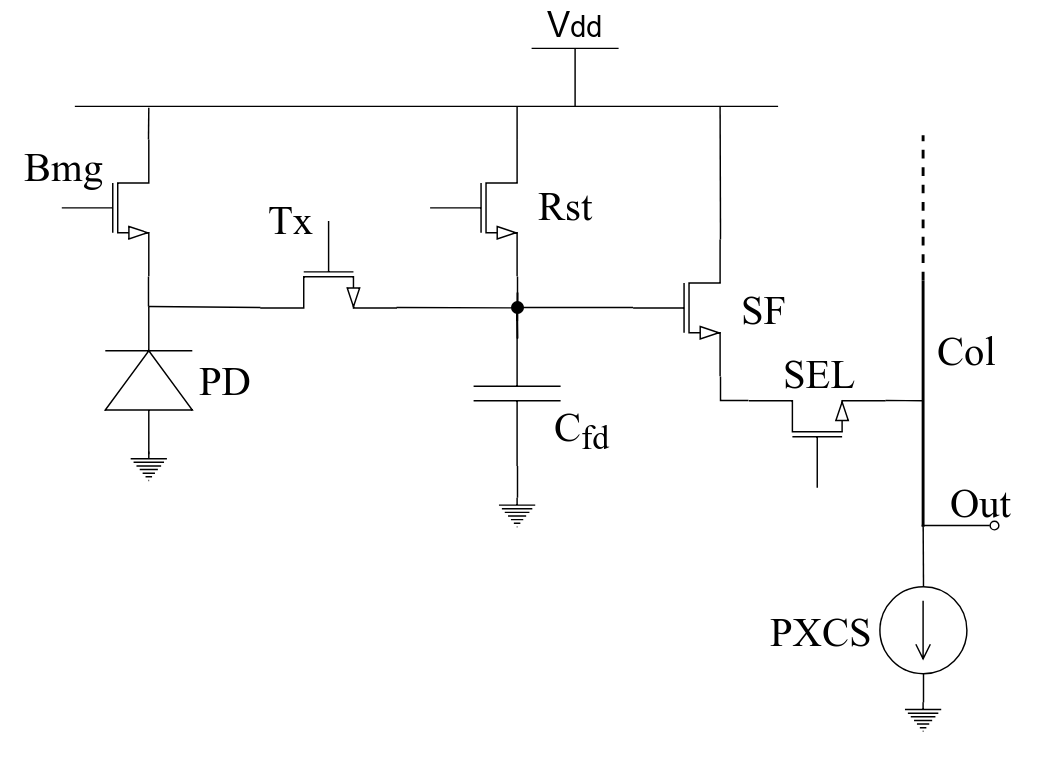
\includegraphics[width=\textwidth]{img/pixel_5T.png}
		\caption{}
		\label{fig:pixel}
	\end{subfigure}

	 %add desired spacing between images, e. g. ~, \quad, \qquad, \hfill etc.
	%(or a blank line to force the subfigure onto a new line)
	\begin{subfigure}{\textwidth}
		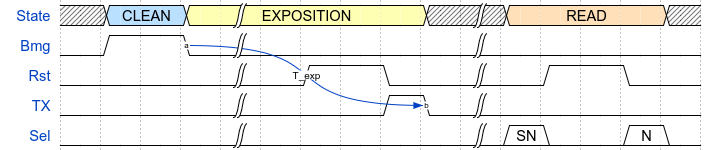
\includegraphics[width=\textwidth]{img/pixel_wave.png}
		\caption{}
		\label{fig:pixel_op}
	\end{subfigure}
	\caption{Esquemático y modo operación de un píxel 5T habitual}
\end{figure}

Mirando el modo de operación (\ref{fig:pixel_op}) vemos que antes de la exposición se hace un vaciado del
fotodiodo mediante el transistor de BMG, que coloca una tensión alta en el fotodiodo.
Durante la exposición, los electrones fotogenerados van bajando la tensión de este
nodo. Para terminar la exposición, se hace una transferencia de esta carga hacia
el condensador $C_{fd}$ (\textit{Floating Diffusion}), no sin antes dar un pulso
en el transistor de RST (Reset), para vaciar la posible carga que tuviera este condensador.\\

En este punto tenemos la carga con la información de la luz captada por el píxel,
almacenada en el condensador $C_{fd}$, a la espera de que queramos leer este valor
mediante la activación del transistor SEL (Selección). Normalmente, para compensar
errores debidos a asimetrias en los píxeles, se hace una operación de CDS, siglas de
``\textit{Correlated Double Sampling}''. Esto es, medir la señal bruta que tenemos
en la ``floating diffusion'', e inmediatamente después, limpiar este condensador con
un pulso de Reset y volver a leer. De esta forma, simbolizando con S, señal y N,
ruido (\textit{noise}), si restamos ambas formas de onda, podemos obtener:

\begin{equation}
	\label{eq:CDS_operation}
	S = SN - N
\end{equation}

Podemos hacer esto debido a que ambas medidas  están correlacionadas porque se
hacen con muy poco tiempo de diferencia y entonces los ruidos son aproximadamente
iguales.\\

Habitualmente existen dos formas de exponer el array: ``\textit{global shutter}'',
obturación global, y ``\textit{rolling shutter}'', obturación consecutiva. En la
primera, todas las filas del array se exponen simultáneamente y luego, fila por fila
se van leyendo los valores almacenados en las ``\textit{floating diffusions}''. En
el segundo caso, la exposición se hace secuencialmente, fila por fila, antes de cada
lectura.\\

La operación de \textit{sampling} y comparación de estas señales se realiza en el
bloque del ADC, que se describirá más abajo en el apartado \ref{cap:ro_sch_adc}.
Existe una interesante técnica para duplicar velocidad de lectura haciéndo
simultáneamente el muestreo de las señales y su comparación con el valor de la rampa.
Ésta técnica de lectura en \textit{pipeline} o también llamada \textit{ping-pong},
requiere duplicar el bloque del ADC por cada columna de píxeles que tengamos. El
siguiente diagrama \ref{fig:ping_pong} de fases muestra su funcionamiento.\\

\begin{figure}[h]
	\centering
	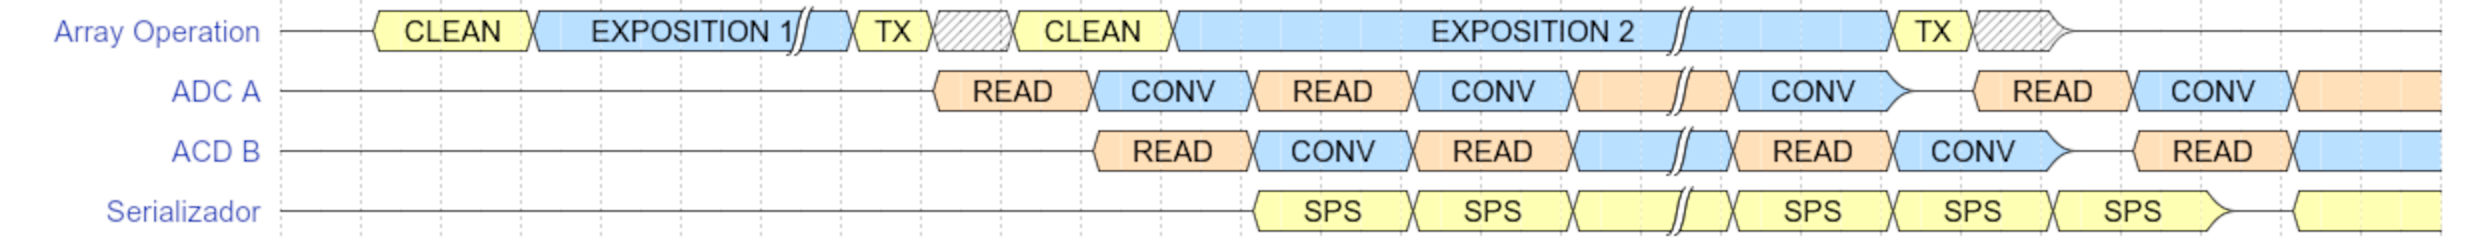
\includegraphics[width=\textwidth]{img/ping-pong_wave.png}
	\caption{Diagrama de fases para la técnica ping-pong con \textit{global-shutter}}
	\label{fig:ping_pong}
\end{figure}


\section{Fuente de corriente}\label{cap:ro_sch_pxcs}

La fuente de corriente, normalmente abreviada como PXCS (del inglés,
\textbf{P}i\textbf{x}el \textbf{C}urrent \textbf{S}ource),
es el primer bloque que se sitúa en
en el canal de lectura y es común a todas las filas de píxeles. Básicamente
es un transistor polarizado en saturación, de modo que drena una corriente
constante que copia de otro transistor con el que forma un espejo de corrientes.
Podemos ver un esquemático del circuito habitual en la figura \ref{fig:pxcs_sch}.\\

Normalmente, la corriente es configurable, para permitir tiempos de lectura menores
incrementando su  valor, o por el contrario, disminuir el consumo si no necesitamos tanta
velocidad.

\begin{figure}[h]
	\centering
	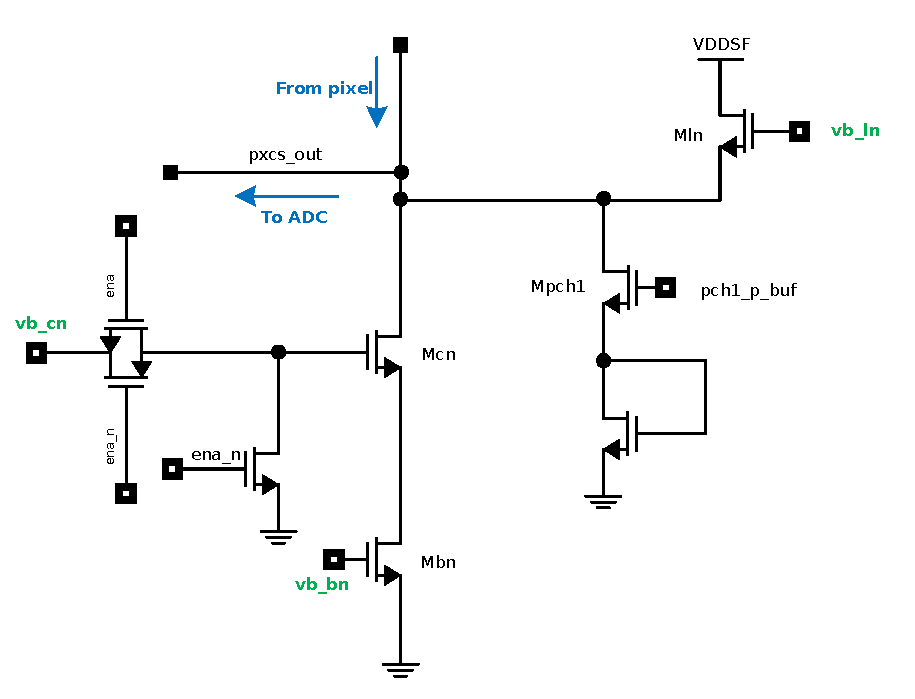
\includegraphics[width=0.8\textwidth]{svg/pxcs_sch.pdf}
	\caption{Esquemático de la fuente de corriente del píxel}
	\label{fig:pxcs_sch}
\end{figure}

La rama que va a tierra desde el nodo de salida del bloque se usa para la pre-carga.
La llamada pre-carga es un sistema que se usa habitualmente para hacer que el
establecimiento de la señal cargada por la fuente de corriente se haga más rápido
y en las mimas condiciones siempre. Lo que se hace es dar un pulso de pre-carga
(\textit{pch}) un poco antes de activar el \textit{sel}. Ésta rama hace bajar la
tensión de salida del píxel a un valor cercano a cero para empezar a evolucionar
desde ahí al valor de la \textit{floating diffusion} menos el $V_{gs}$ del seguidor
por fuente (SF) del píxel.\\
%WARNING
%Continuar aquí y explicar mejor precarga y limitador

\section{ADC}\label{cap:ro_sch_adc}

Como ya hemos comentado, la conversión del valor analógico del píxel, a un número
digital se realiza mediante un convertidor de rampa. Para conseguir esto,
en cada canal de lectura se implementa un sencillo ADC comparador y unos condensadores
dónde almacenar temporalmente las señales.\\

La señal de la rampa analógica se va a distribuir horizontalmente entre todas las
columnas del canal de lectura, y está generada por un bloque externo al RO, situado
a uno de los lados del mismo, con lo que evitamos incluirlo en area del canal.\\

El ADC es el bloque que \textbf{muestrea} y \textbf{compara} la señal analógica del píxel con la de la
rampa analógica. El esquemático del circuito se muestra en la figura \ref{fig:adc_sch}.
La operación del ADC se realiza en 2 fases, lectura (\textit{read}) y comparación
(\textit{comp}), y se puede seguir mediante las formas de onda mostradas en \ref{fig:adc_wave}.\\

\begin{figure}[h]
	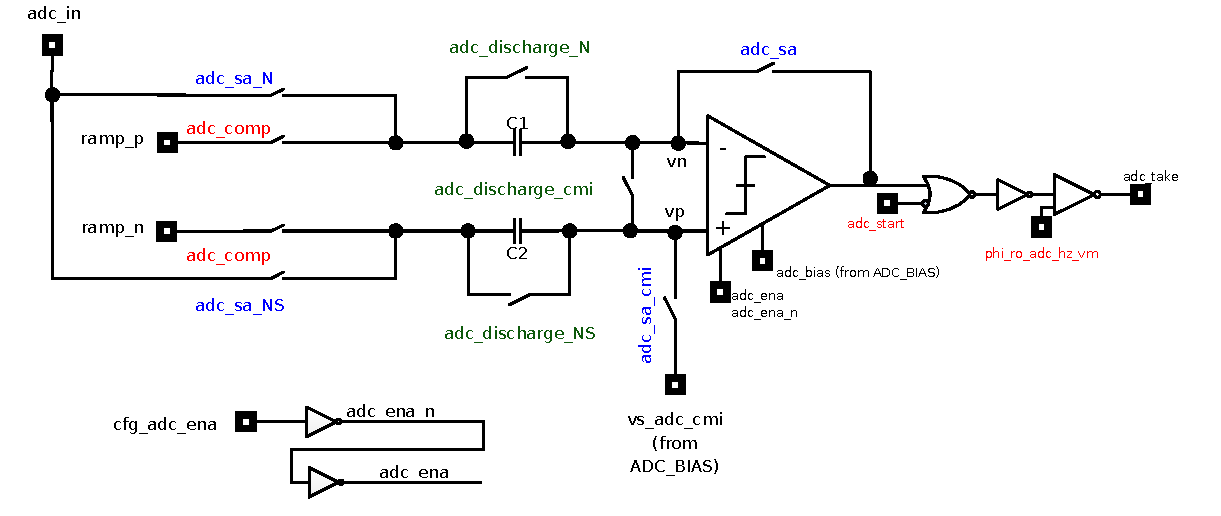
\includegraphics[width=\textwidth]{svg/adc_sch.pdf}
	\caption{Esquemático del ADC}
	\label{fig:adc_sch}
\end{figure}

\begin{figure}[h]
	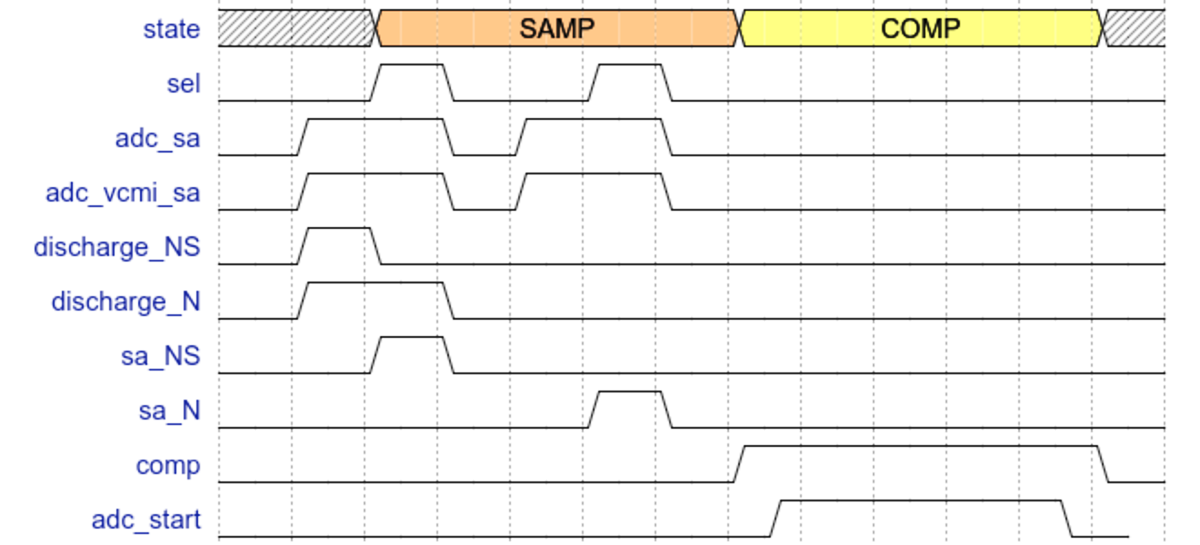
\includegraphics[width=\textwidth]{img/adc_wave.png}
	\caption{Señales de onda del comparador de rampa}
	\label{fig:adc_wave}
\end{figure}

Durante la primera de ellas, el comparador está operando en lazo cerrado, por lo
los nodos de entrada $vp$ y $vn$ se establecen a la tensión de modo
común, $vs\_adc\_cmi$. Al final del periodo de muestreo, las señales
``señal + ruido'' (NS) y ``ruido'' (N), quedan almacenadas en los condensadores $C_2$
y $C_1$, respectivamente.\\

En la segunda fase, el comparador se establece en lazo abierto, por lo que la carga
almacenada en los condensadores se mantiene. En ese momento se conecta la
rampa diferencial ($ramp_P$ y $ramp_N$), y aplicando la conservación de carga en los
nudos $vp$ y $vn$, se puede deducir que el voltage será:\\

\begin{align}
	v_n &= \dfrac{v_{cmi} + v_{off}}{1+\frac{1}{A_0}} + \alpha_1 (v_{ramp_p}-v_{pixN})\\
	v_p &= v_{cmi} + \alpha_2 (v_{ramp_n}-v_{pixNS})
\end{align}
, dónde los coeficientes $\alpha_1$ y $\alpha_2$ son:\\

\begin{equation}
	\alpha_1 = \dfrac{C_1}{C_1+C_p},~
	\alpha_2 = \dfrac{C_2}{C_2+C_p}
\end{equation}

Asumiendo un comparador ideal, el voltage diferencial a la entrada de este, se
puede expresar como:\\

\begin{equation}
	\Delta V= v_p - v_n = (v_{pixNS}-v_{pixNS}) - (v_{ramp_p}-v_{ramp_n})
\end{equation}
, dónde la diferencia $(v_{pixNS}-v_{pixNS})$ es siempre positiva y se relaciona
con la información almacenada en el píxel, y la señal $(v_{ramp_p}-v_{ramp_n})$ es
linealmente creciente. Por tanto, la salida del comparador debe ser inicialmente
un valor alto y cambiar a valor bajo en el instante en que ambas señales sea crucen.
Por lo que la información en el píxel puede codificarse con el tiempo registrado
por un contador digital, siendo mayor el número digital a mayor la luz recibida
por el píxel leído.

La salida del comparador se hace pasar por una puerta NOR para evitar que pueda
registrarse una transición sin estar activa la señal de $adc\_start$\\

\subsection{OTA}\label{cap:ro_sch_ota}

El OTA (\textit{Operational Transconductance Amplifier}) es el bloque que actúa
cómo comparador y tiene la estructura de un amplificador diferencial simple, que
se muestra en el esquemático de la figura \ref{fig:ota_sch}.\\

\begin{figure}[h]
	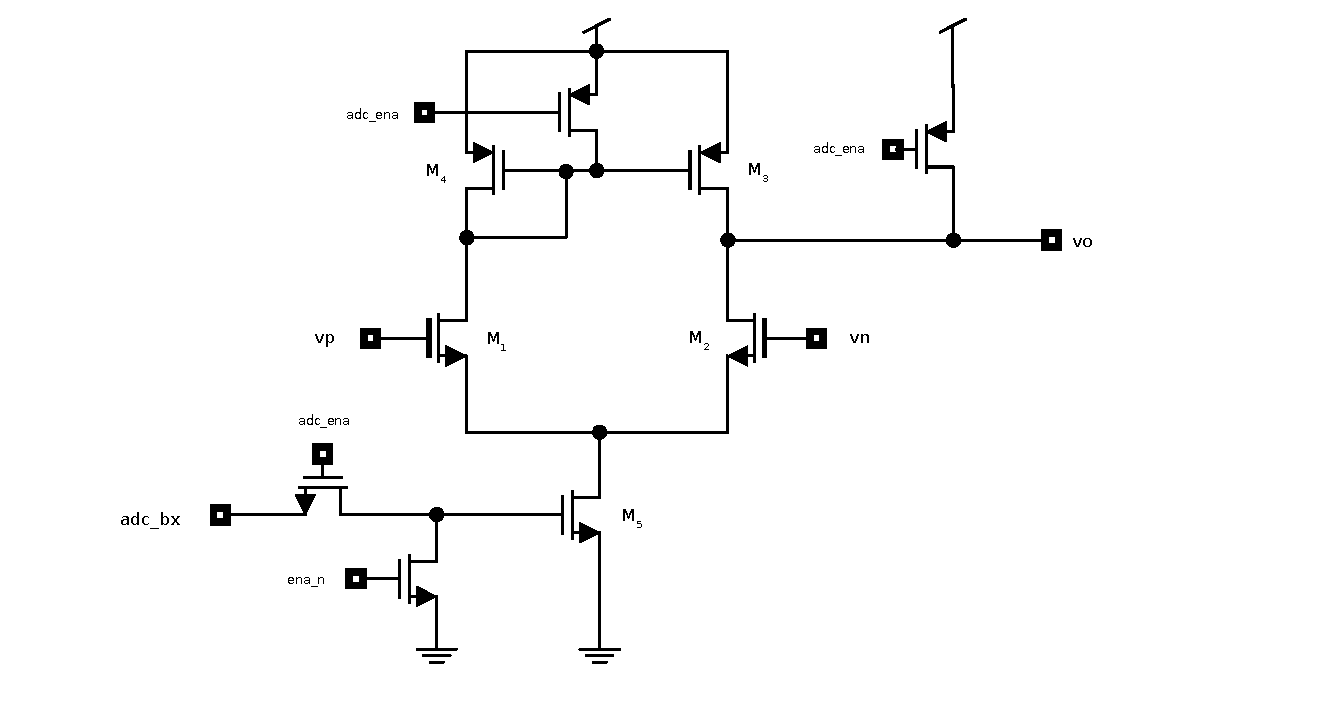
\includegraphics[width=\textwidth]{svg/ota_sch.pdf}
	\caption{Esquemático del OTA comparador}
	\label{fig:ota_sch}
\end{figure}

Los transistores $M_1$ y $M_2$ forman el par diferencial, con sus correspondiente
espejo de corrientes en $M_3$ y $M_4$, y la fuente de corriente $M_5$, el resto de
transistores sirven para deshabilitar el OTA cuando no se esté usando.\\

\section{Generador de rampa analógica}\label{cap:ro_sch_armp}

El bloque generador de la rampa analógica se encuentra situado fuera del Canal de
Lectura. Se encarga de generar una señal linealmente creciente y su correspondiente
decreciente. El rango en el que la rampa varía debe ajustarse en fucnión del rango
de entrada del OTA del comparador y teniendo en cuenta el rango en el que varía
la salida del píxel, para obtener una resolución deseada y aprovechar al máximo
la sensibilidad del sensor.\\

Es muy importante una precisa generación de ésta rampa analógica, con especial
atención a la linealidad de la misma. En la bibliografía se describe una arquitectura
para el generador de rampa que obtiene una buena linealidad por debajo de un LSB
para resoluciones de hasta 15 bits a frecuencias de reloj de 100MHz\cite{Sordo-Ibanez2013},
que está en un rango adecuado para los tiempos de lectura que se suelen tratar en
sensores de imagen CMOS.\\

La señal generada debe propagarse a lo largo de lo todos los canales de lectura,
desde la izquierda hacia la derecha, o al contrario, en su caso. Para conseguir
una rápida y efectiva propagación de esta señal sin distorsión y en tiempo, ha
de hacerse un cuidadoso estudio de layout, calculando las anchuras y separaciones
entre las líneas metálicas que distribuirán la señal y posteriormente, realizando
una precisa extracción y simulación del circuito.\\

\section{Bloques de polarización}\label{cap:ro_sch_bias}

Los bloques del canal descritos anteriormente, la fuente de corriente y el ADC
requieren de varias señales de polarización, que habitualmente, además, suelen
ser programables, esto es, que permiten diferentes valores de configuración
establecidos por el usuario del dispositivo sobre pr ejemplo, la velocidad de
lectura, la resolución deseada, el consumo.\\

Normalmente, para ahorrar espacio, los bloques de polarización, o \textit{BIAS},
se comparten entre varios canales de lectura. De esta forma, el layout de estos
bloques puede ser más ancho que alto, con lo que conseguimos un ahorro de área en
la dirección vertical.\\

\subsection{PXCS Bias}

La fuente de corriente necesita de tres voltajes de polarización: $vb\_bn$ y
$vb\_cn$, que vienen de un espejo cascodado y la tensión del limitador $vb\_ln$.
El bloque va a estar compartido por 8 canales (80$\mum$ de anchura).\\

Los valores de la corriente que podrá drenar la fuente de corriente del píxel, va
a ser configurable con 5 bits de resolución. Ésta configuración será implementada
en este bloque de polarización mediante 5 ramas de corrientes que conduzcan,
respectivamente, $I_0$, $2I_0$, $2I_0$, $4I_0$, $8I_0$, con
$I_0=125\nA$. De forma que podemos variar la corriente total entre $125\nA$ y
$3.875\muA$, en pasos de $125\nA$.\\

\subsection{ADC Bias}

El ADC Bias tiene que proveer al ADC del voltaje de modo común ($vs\_adc\_cmi$) y
de la tensión de bias de la fuente de corriente del OTA ($vb\_adc\_bx$), que espejará
una corriente generada en el Bias.\\

La tensión de modo común se puede generar de dos formas, la primera mediante un
buffer que replica una tensión generada en el bloque de Referencias, fuera del
canal de lectura, y la segunda generando un tensión local por cada grupo de canales.
Ésta segunda opción también usa una referencia común, pero al ser local, se adapta
mejor a la eventual curva en las alimentaciones que podremos tener a lo largo
del RO. Éste tema se tratará con más detalle en la correspondiente sección de layout.\\

\section{Rampa digital y serialización}

Una vez la operación de comparación se ha iniciado, la rampa y la señal del píxel,
en algún momento se cruzarán, lo que desencadenará una transición en la señal
$adc\_take$ que es la que finalmente sale de la parte analógica del canal y se va
a rutar hacia abajo para ser registrada por el contador digital.\\

Dicho contador (o rampa) digital habrá empezado la cuenta desde cero, en un tiempo y a una
velocidad adecuados para que el valor más alto de la cuenta digital (la resolución)
coincida con el valor final de la rampa analógica y con el valor mínimo de tensión
de salida del píxel (máxima intensidad lumínica). En el momento en que se recibe
el pulso en la salida $adc\_take$, se detiene la cuenta digital y tenemos un valor
digitalizado proporcional a la intensidad lumínica captada por el píxel actual.\\

El bloque que genera la rampa digital DRMP se sitúa a uno de los lados del RO y
su señal se distribuye mediante búferes digitales a lo largo del SPS, que es
el bloque digital situado justo debajo del Canal de Lectura y que incluye la digitalización
y serialización de los datos.\\

La serialización se efectúa para convertir la operación de digitalización, que se
hace de forma paralela, simulatánea a todos los canales, a una salida de datos en serie.
Éstos datos en serie se encaminan posteriormente hacia uno o varios buses de salida LVDS
(\textit{Low Voltage Differential Signal}), que harán posible la lectura de las imágenes
desde el exterior.\\

\chapter{Diseño del layout de un canal de lectura}

El diseño del layout de un canal de lectura en el contexto de un proyecto suele
ser una tarea que ocupa gran parte del periodo de diseño, y además es recomendable
abordar en las primeras fases del proyecto, ya que como hemos comentado, el
layout va a influir, en mayor medida que otros bloques, en el diseño del mismo.
Por tanto, el diseño del canal de lectura suele ser un proceso iterativo de
diseño electrónico, layout, extracción, simulación y eventual rediseño.\\

\section{Jerarquización}

A la hora de estructurar el diseño de layout de cualquier bloque repetitivo, como
es el canal de lectura, es básico idear una estrategia en cuanto a la jerarquización
del mismo, ya que usualmente no se trata de un simple array de instancias iguales
situadas una al lado de la otra.\\

Por otra parte, existen estructuras que pueden requerir diferentes periodicidades.
Y también hay que adaptarse a la resolución del array, en este caso, al número de
columnas. Cómo ya hemos visto a lo largo de la descripción del esqumático del canal
nuestra unidad básica de un canal de lectura, a la que nos referiremos como
$ro\_chx1$, ocupará una anchura de 2 columnas de píxeles, es decir, una anchura
de $10\mum$. En esa anchura tiene que ser posible incluir todos los bloques que
se repiten por canal, es decir, la fuente de corriente y el ADC de una columna de
píxeles.\\

En un siguiente nivel de jerarquía, incluiremos 8 canales unitarios y sus
correspondientes bloques de polarización (PXCS\_BIAS y ADC\_BIAS), que cómo vimos
están compartidos por cada 8 canales. De ésta forma, el bloque $ro\_chx8$
tendría una anchura de $10\mum \times 8 = 80\mum$, y tendríamos canales para
leer 16 columnas de píxeles.\\

Desde 16 columnas hasta las columnas totales del array podemos elegir varios niveles
de jerarquías intermedios. Considerando que nuestro array tiene la estructura
mostrada en el capítulo \ref{cap:pxa_array}, en la figura \ref{fig:pxa_array},
con 2560 columnas activas y 64 columnas oscuras, vamos a hacer una jerarquía que
cubra esos 64 píxeles, es decir, 32 canales, por lo que se llamará $ro\_chx32$ e
instanciará 4 unidades de $ro\_chx8$.\\

Para completar las 2560 columnas de píxeles activos, sólo hay que instanciar 40
de los bloques de 32 canales. Y para completar el array, tan sólo hay que añadir
2 canales (4 píxeles) a izquierda y derecha de la zona activa (píxeles dummy), y
un bloque de 32 canales en la zona de las columnas oscuras, con sendos pares de
canales a izquierda y derecha para hacer las columnas oscuras dummy.\\

\subsection{Redundancia}

En todo diseño microelectrónico, debido a defectos en la fabricación, ciertos
dispositivos pueden resultar completamente inutilizables o, al menos, con prestaciones
por debajo de lo esperado en relación al resto de dispositivos equivalentes.
Ésto se acentua en casos como un canal de lectura, en los cuales la integración
y la congestión de rutado y dispositivos es muy alta, y además tiene un patrón
altamente simétrico y periódico.\\

Con el paso del tiempo, los fabricantes de sensores de imágen han detectado que
el canal de lectura sufre de considerablemente más fallos que el resto de circuitos
en el sensor, y por consiguiente es uno de los principales contribuyentes a la
disminución del ``\textit{yield}'' (del inglés: rendimiento), que da cuenta del
porcentaje de sensores por oblea que no funcionan o son defectuosos, lo que va
en contra del beneficio económico.\\

Para tratar de disminuir éste problema, se suele poner en práctica el uso de canales
redundantes, ésto es, canales adicionales que podrían ser usados en el caso de que,
una vez fabricado el chip, se detecten fallos en un canal concreto.\\

Para ésto se añade un canal adicional cada cierto número de canales y mediante un
sistema de llaves a la entrada de todos los canales podemos redireccionar la
salida todos los píxeles en el rango afectado y posteriores al canal del fallo,
hacia el siguiente canal. Con ésto se puede ver fácilmente que podemos solucionar
tantos fallos como canales redundantes sean incluidos, siempre y cuando no se
produzca más de un fallo por región.\\

\begin{figure}[h]
	\includesvg[width=\textwidth]{svg/redundancy.svg}
	\caption{Ejemplo del funcionamiento del sistema de redundancia}
	\label{fig:redundancy}
\end{figure}

En la figura \ref{fig:redundancy} vemos un ejemplo de aplicación del sistema de
redundancia dónde tendríamos un canal redundante por cada 4. En el que caso de que
fallen los canales 2 y 5 mostrados en la imagen, el bloque de redundancia colocado
en la parte superior del canal de lectura podría dirigir cada columna a la siguiente,
de la forma que muestran las líneas rojas.\\

Cómo ya se puede intuir, la anchura del canal de lectura, en el supuesto de usar
redundancia se tiene que ver reducida con objeto de incluir un canal adicional
cada cierto tiempo. En nuestro caso vamos a incluir un canal redundante por cada
grupo de 32 canales funcionando. Con ésto, haciendo una sencilla cuenta, podemos
establecer la nueva anchura en $9\mum$ en vez de las $10\mum$ originales. Ésto nos
permite además tener una anchura sobrante cada 33 canales que será:
$32\cdot 10\mum - 33\cdot 23\mum = 23\mum$ de anchura sobrante. Este espacio lo
podemos usar para por ejemplo subir las tensiones de polarización desde los BIAS
a las líneas horizontales en los correspondientes bloques.\\

\section{Estructura de layout de una columna del canal}

Una vez establecida una jerarquía clara, y suponiendo el uso de la redundancia ya
tenemos establecida una anchura para el layout de una columna de nuestro canal.
En ésta anchura deberemos incluir todos los bloques descritos en el esquemático
tratando de hacerlo lo más compacto posible para ahorrar área en la dirección vertical.\\

Cómo hemos introducido en el apartado anterior, el bloque de redundancia será
el primero que nos encontraremos por la parte superior, más cerca del array de
píxeles. Para ésto además tiene que existir un rutado que transforme las salidas
de los píxeles, espaciadas cada $5\mum$ a las entradas de los bloques de redundancia,
espaciadas 2 cada $9\mum$.\\

Lo siguiente que tenemos es la fuente de corriente, que es una por cada columna
de píxeles, es decir, dos en cada canal unitario, y se van a colocar una encima
de otra ocupando ambas la anchura del canal, $9\mum$.\\

Inmediatamente debajo colocaremos el bloque de polarización de las fuentes de
corriente, PXCS\_BIAS, que como se comparte para 8 canales, en la unidad $ro\_chx1$,
dejaremos un hueco de la altura necesaria, que se establecerá en función de la altura
del BIAS.\\

Por debajo del PXCS\_BIAS, vamos a colocar los ADC, que tiene que haber dos por
cada columna de píxeles si queremos usar la técnica de ping-pong. En nuestro caso
esto significa tener que implementar 4 ADCs idénticos dispuestos en vertical ocupando
las $9\mum$ de anchura del canal.\\

Por último, bajo los 4 convertidores iría el Bias del ADC, que tambíen se comparte
por cada 8 canales, por lo que tampoco estaría incluida en columna unitaria.\\

\section{Problemas de layout que afectan al diseño del canal de lectura}

\subsection{Consumo}

El consumo de un bloque tan grande como es el canal de lectura siempre es algo a
tener muy en cuenta a la hora de modelar las alimentaciones que debe tener y
cómo afectan éstas al funcionamiento del propio bloque y del resto del sensor.\\

En muchas ocasiones no es tan importante que un bloque tenga un consumo alto,
cómo la dinámica con la que se produzca ese consumo. Si un bloque tiene un alto
consumo, pero lo hace de manera más contínua que otro que tiene grandes picos de
alto, quizás afecte menos al rendimiento total del circuito. En el caso del
canal de lectura esto es muy importante porque muchos de los procesos se producen
de forma simultánea en todos los canales a la vez. Por esta razón hay que tener
especial cuidado a cómo se programan los tiempos de lectura y comparación,
y, lo más importante, realizar exhaustivas simulaciones usando extraído de parásitos
y modelando muy bien las alimentaciones y los acoplos que podemos tener. Este tema
se tratará en más detalle en el apartado \ref{cap:simulacion} sobre simulaciones.\\

Otro punto importante a considerar es que el canal de lectura va a ser alimentado,
tan sólo por ambos extremos. Ésto va a generar una curvatura en las alimentaciones
que puede traer problemas, manifestándose como un gradiente en la imágen final.
Las tensiones de polarización del los bloques de bias, están generadas localmente
y referidas a una tierra con curvatura por lo que unos ADC y otros
podrían tener tener diferente tiempo de conversión, por ejemplo.\\

\begin{figure}[h]
	\includesvg[width=\textwidth]{svg/adc_poly_short.svg}
	\caption{Curvatura en la tensión de tierra y una tensión de polarización a lo largo del canal}
	\label{fig:adc_poly_short}
\end{figure}

Para tratar de corregir éste efecto, se suelen cortocircuitar las tensiones de polarización
entre todos los canales del array. En la imágen \ref{fig:adc_poly_short} podemos ver
3 casos. El caso (a) lo que ocurriría si no cortocircuitamos los adc\_bias,
el caso (b), si lo hacemos con una línea metálica, con baja resistividad,
y el caso (c) si lo hacemos con una línea más resistiva, de poly.
La solución elegida es la última porque suaviza mucho mejor los voltajes de polarización
entre los diferentes canales, al adaptarse a la irremediable curvatura de la tierra.\\

\subsection{Acoplos}

Otro tema crítico en el diseño del layout del canal de lectura es los posibles acoplos
entre señales debidos principalmente a la apilación de canales requerida por la
paralelización de varios píxeles y por el uso de la técnica de ping-pong. Es más,
el uso del ping-pong hace incluso más crítico éste tema, ya que va a significar
que en los mismos periodos de tiempo van a concurrir fases de muestreo y comparación
en canales que se encuentran apilados.\\

Algunas líneas como el $adc\_take$ que saldría de un canal superior, va a tener que,
obligatoriamente, pasar por encima de algún canal inferior que esté haciendo
\textit{sampling}. Y, debido a que la transición del \textit{take}, se produce
en un momento indeterminado, en función de la luz captada por el píxel leído, puede
coincidir que dicha transición se produzca en el periodo final de una fase de
muestreo del otro canal. Si ésta señal tiene un acoplo con uno de los nodos de
entrada del comparador, o con los condensadores, puede ocurrir que se produzca
un pico en la señal que se está muestreando y al ser el final del periodo de muestreo,
no dar tiempo a que se reestablezca y haber finalmente modificado el valor leído.\\
%WARNING
%Revisar expresion de este ultimo parrafo (simplificar si se puede)

\subsection{Condensadores del ADC}

Los dos condensadores que debe haber por cada ADC son otro punto a tener en
consideración, ya que son una parte fundamental del mismo. Lo primero que
hay que decir es que suelen ser grandes, más aún si se trata de un sensor de
bajo ruido, ésto es, que está destinado a captar imágenes con escasa iluminación
y se requieren altos rango dinámico y resolución, por lo que se necesitan condensadores
mayores.\\

También son grandes porque habitualmente se implementan usando condensadores
metálicos, que usan placas de metal 3 y 4 una sobre la otra. Éste tipo de condensador
tiene una densidad de capacidad por unidad de área menor que otros como los tipo
MOS descritos en \ref{cap:condensadores}, pero se usan por la mayor linealidad que
éstos últimos.\\

Un punto a tener atención es al apantallado de éstos condensadores entre los de
las columnas vecinas. Si entre ellos hubiera una capacidad alta, podría haber
una transferencia de carga si el valor almacenado en uno de ellos es muy diferente
al otro, lo que crearía un efecto de desenfoque de los bordes abruptos en la imagen.\\

Otro problema que introducen los condensadores, en concreto, que estén fabricados
los metales superiores 3 y 4, es que las señales que se distribuyen verticalmente,
cómo el $adc\_take$ y la salida del píxel, que habitualmente se rutan en los metales
más altos para facilitar el apantallado, van a tener que bajar para pasar por debajo
de los condensadores. Ésto va a posibilitar que se acoplen a otras señales que se ruten
en metales inferiores.\\

\subsection{Distribución de señales horizontalmente}

Cómo ya se ha comentado en otros apartados, la distribución horizontal de las
señales de control, o \textit{fases}, necesita especial atención, sobre todo
si el array consta de muchas columnas.\\

Una de las principales señales horizontales es la rampa analógica. En el caso de
producirse un retraso en la propagación de ésta, los valores leídos serían mayores
de los verdaderos. Por lo tanto siempre trataremos de disminuir dicho tiempo de
propagación, lo que se consigue con baja resistencia, esto es, mayor anchura de
líneas, y menor capacidad, mayor espaciado con otras líneas o con el substrato.
Por otra parte, es bueno que no se ensucie con posibles acoplos con señales verticales,
por lo que habitualmente se elige rutar la rampa en metal Top de $10\mum$ de anchura,
sobre una capa de Metal 3 conectado a tierra como apantallamiento.\\

Siempre y cuando el error producido por el retraso de la rampa quede por debajo
de un LSB, no se vería nada en la imágen debido a éste retraso. Si no es así, y es
inevitable un pequeño retraso, siempre se puede corregir posteriormente, ya que
se trata de un error de patrón fijo \textit{``Fixed Pattern Noise''} o FPN, que
en la fase de caracterización del sensor, se podría corregir mediante unos
parámetros de ajuste por canal.\\

En cuanto a los retrasos en las fases, como éstos afectan a las señales de
muestreo, debemos tener más cuidado puesto que podría darse el caso extremo de
que las fases de muestreo se descuadren demasiado con la señal de \textit{sel} del
píxel y que perdamos periodo de muestreo efectivo. Ésto se debe corregir tratando
de ecualizar la constante de tiempo la señal de \textit{sel} con el resto de
fases. Hay que recordar que normalmente la primera tiene mucha menos libertad a la
hora del diseño. La anchura y la capacidad del \textit{sel} está muy acotada
por el complejo diseño del layout del píxel. Por lo tanto sólo podemos actuar
sobre el diseño de las líneas de las fases del canal. Debemos comprobar bien
anchuras, acoplos a otras líneas y tamaño y cantidad de dispositivos que cuelgan
de ellas, tratando de equilibrar las constantes de tiempo de todas ellas.\\

Para ésto, una vez más, es muy importante una cuidada extracción de parásitos y
exhaustivas simulaciones post-layout, en diferentes canales a lo largo de todo el
array.\\

\section{Bloques adicionales}

\subsection{Binning}

Con el nombre de \textit{binning} nos referimos a una técnica de combinación de
varios píxeles en uno sólo, de forma que reducimos la resolución efectiva del
array y podemos leerlo más rápido. Normalmente se pueden combinar grupos de
$2\times 2$ o $4\times 4$ píxeles.\\

El binning se puede implementar posteriormente a nivel digital o en el propio
canal de lectura.\\
%WARNING
%Completar con algo de binning

\subsection{Implementación de ROIs}

Una ROI, del inglés \textbf{R}egion \textbf{O}f \textbf{I}nterest, es una zona
de la imagen que el usuario puede seleccionar para leer, obviando el resto
del array. Con ésto podríamos disminuir el tiempo de lectura, sólo si
disminuye el numero de filas.\\

Otra ventaja para usar una ROI sería que podríamos desactivar los canales que no
estén usando, con lo que disminuiría el consumo total del chip. Para ésto debemos
tener un control por deshabilitación de los canales por columnas, o al menos, por
grupos de columnas, por ejemplo una buena estrategia sería poder desactivar cada
BIAS y con ellos, los correspondientes 8 canales, o 16 píxeles.\\

\chapter{Conclusiones}

\section{Dificultad creciente de los canales de lectura}

\section{Condicionamiento del diseño del canal por aspectos de layout}

\section{Estudios de viabilidad adecuados}

\section{Uso de nuevas tecnologías}

\section{Innovaciones en las tecnologías de los píxeles}

\bibliography{doc/TFG}
\bibliographystyle{plain}


\end{document}
